\documentclass[12pt]{article}

\usepackage{sbc-template}

\usepackage{graphicx,url}
\usepackage{float}
\usepackage[brazil]{babel}   
%\usepackage[latin1]{inputenc}  
\usepackage[utf8]{inputenc}  
% UTF-8 encoding is recommended by ShareLaTex
\usepackage{xcolor}
% Definindo novas cores
\definecolor{verde}{rgb}{0.25,0.5,0.35}
\definecolor{jpurple}{rgb}{0.5,0,0.35}
% Configurando layout para mostrar codigos Java
\usepackage{listings}
\lstset{
	language=Java,
	basicstyle=\ttfamily\small, 
	keywordstyle=\color{jpurple}\bfseries,
	stringstyle=\color{red},
	commentstyle=\color{verde},
	morecomment=[s][\color{blue}]{/**}{*/},
	extendedchars=true, 
	showspaces=false, 
	showstringspaces=false, 
	numbers=left,
	numberstyle=\tiny,
	breaklines=true, 
	backgroundcolor=\color{cyan!10}, 
	breakautoindent=true, 
	captionpos=b,
	xleftmargin=0pt,
	tabsize=4
}
\pagestyle{empty}
     
\sloppy

\title{Sistma Gerenciador de FTP \\ Exercício Computacional I}

\author{Rafael Gonçalves de Oliveria Vianal\inst{1} }


\address{Sistemas de Informação -- Universidade Federal do Mato Grosso do Sul
	(UFMS)\\
  	Caixa Postal 79400-000 -- Coxim -- MS -- Brazil
  \email{rafael.viana@aluno.ufms.br}
}

\begin{document} 

\maketitle

     
\begin{resumo} 
  Este relatório descreve como foi construido um sistema gerenciador de FTP, utilizando JavaFx como \textit{Graphical User Interface} e o Apache Commons Net 3.6, como biblioteca de conexão FTP.
\end{resumo}


\section{JavaFx}

Foi escolhido o JavaFx para criar uma interface gráfica onde o usuário terá um melhor desempenho, ao utilizar o sistema.
Para criar um sistema elegante foi utilizado uma biblioteca com novos elementos CSS, a bibliteca utilizada para essa finalidade foi  \textbf{JFoenix}, essa bibliteca é open sorce e pode ser baixada no github https://github.com/jfoenixadmin/JFoenix
Para icones foi utilizado a biblioteca fontawesomefx-8.9 
	
\section{Apache Commons Net 3.6} \label{sec:firstpage}

	Para melhor desempenho nas conexões ftp, foi utilizada a biblioteca de conexão FTP da Apache Commons, onde a mesma se encontra na versão 3.6 current.

\section{Problematica}

U

\section{Sections and Paragraphs}

Section titles must be in boldface, 13pt, flush left. There should be an extra
12 pt of space before each title. Section numbering is optional. The first
paragraph of each section should not be indented, while the first lines of
subsequent paragraphs should be indented by 1.27 cm.

\subsection{Subsections}

The subsection titles must be in boldface, 12pt, flush left.

\section{Figures and Captions}\label{sec:figs}


Figure and table captions should be centered if less than one line
(Figure~\ref{fig:exampleFig1}), otherwise justified and indented by 0.8cm on
both margins, as shown in Figure~\ref{fig:exampleFig2}. The caption font must
be Helvetica, 10 point, boldface, with 6 points of space before and after each
caption.

\begin{figure}[ht]
\centering
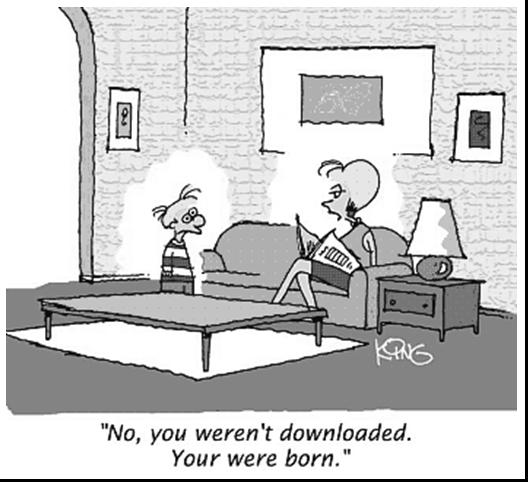
\includegraphics[width=.5\textwidth]{fig1.jpg}
\caption{A typical figure}
\label{fig:exampleFig1}
\end{figure}

\begin{figure}[ht]
\centering
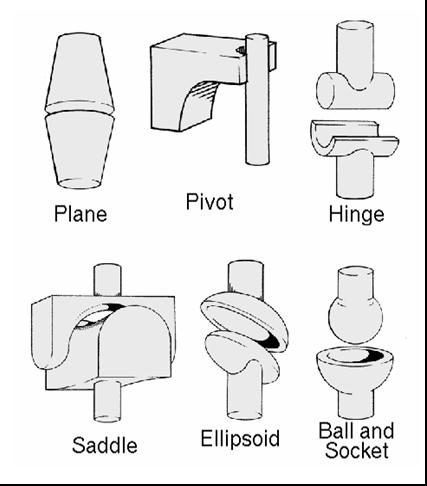
\includegraphics[width=.3\textwidth]{fig2.jpg}
\caption{This figure is an example of a figure caption taking more than one
  line and justified considering margins mentioned in Section~\ref{sec:figs}.}
\label{fig:exampleFig2}
\end{figure}

In tables, try to avoid the use of colored or shaded backgrounds, and avoid
thick, doubled, or unnecessary framing lines. When reporting empirical data,
do not use more decimal digits than warranted by their precision and
reproducibility. Table caption must be placed before the table (see Table 1)
and the font used must also be Helvetica, 10 point, boldface, with 6 points of
space before and after each caption.

\begin{table}[ht]
\centering
\caption{Variables to be considered on the evaluation of interaction
  techniques}
\label{tab:exTable1}
\smallskip
\begin{tabular}{|l|c|c|}
\hline
& Value 1 & Value 2\\[0.5ex]
\hline
&&\\[-2ex]
Case 1 & 1.0 $\pm$ 0.1 & 1.75$\times$10$^{-5}$ $\pm$ 5$\times$10$^{-7}$\\[0.5ex]
\hline
&&\\[-2ex]
Case 2 & 0.003(1) & 100.0\\[0.5ex]
\hline
\end{tabular}
\end{table}

\section{Images}

All images and illustrations should be in black-and-white, or gray tones,
excepting for the papers that will be electronically available (on CD-ROMs,
internet, etc.). The image resolution on paper should be about 600 dpi for
black-and-white images, and 150-300 dpi for grayscale images.  Do not include
images with excessive resolution, as they may take hours to print, without any
visible difference in the result. 

\section{References}

Bibliographic references must be unambiguous and uniform.  We recommend giving
the author names references in brackets, e.g. \cite{knuth:84},
\cite{boulic:91}, and \cite{smith:99}.

The references must be listed using 12 point font size, with 6 points of space
before each reference. The first line of each reference should not be
indented, while the subsequent should be indented by 0.5 cm.

\bibliographystyle{sbc}
\bibliography{sbc-template}

\section{Anexos}

A estrutura do código foi dividida em 3 pastas sendo elas Cliente, Icons e Socket.

 \subsection{A pasta cliente é responsável pela parte de Interface Gráfica do Usuário.}
 \subsection{A pasta Icons armazena icons utilizados na pasta cliente.}
 \subsection{A pasta socket e responsável por toda comunicação da Lib da Apache com o código.}


\begin{figure}[H]
	\centering
	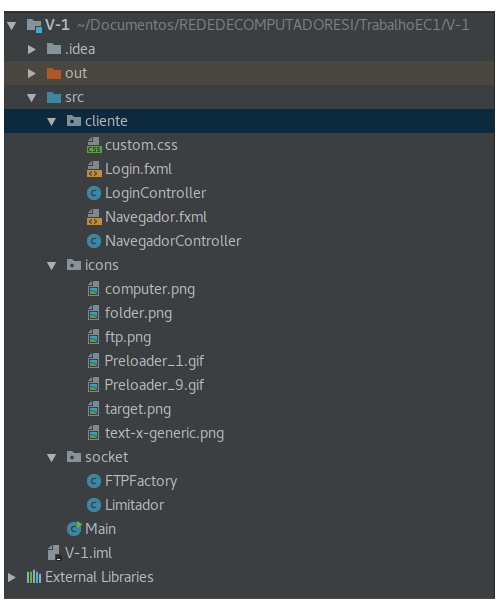
\includegraphics[width=1\textwidth]{Imagens/001.png}
	\caption{ Imagem da Tela de Login.}
	\label{fig:01}
\end{figure}


Primeiramente a Class Main e invocada, chamando a Scene do Login.fxml.

\begin{lstlisting}

public class Main  extends Application{

@Override
	public void start(Stage stage) throws Exception {
	Parent root = FXMLLoader.load(getClass().getResource("/cliente/Login.fxml"));
	Scene scene = new Scene(root);
	stage.setScene(scene);
	stage.show();
}


public static void main(String[] args) {
	launch(args);

}

}

\end{lstlisting}

\begin{figure}[H]
	\centering
	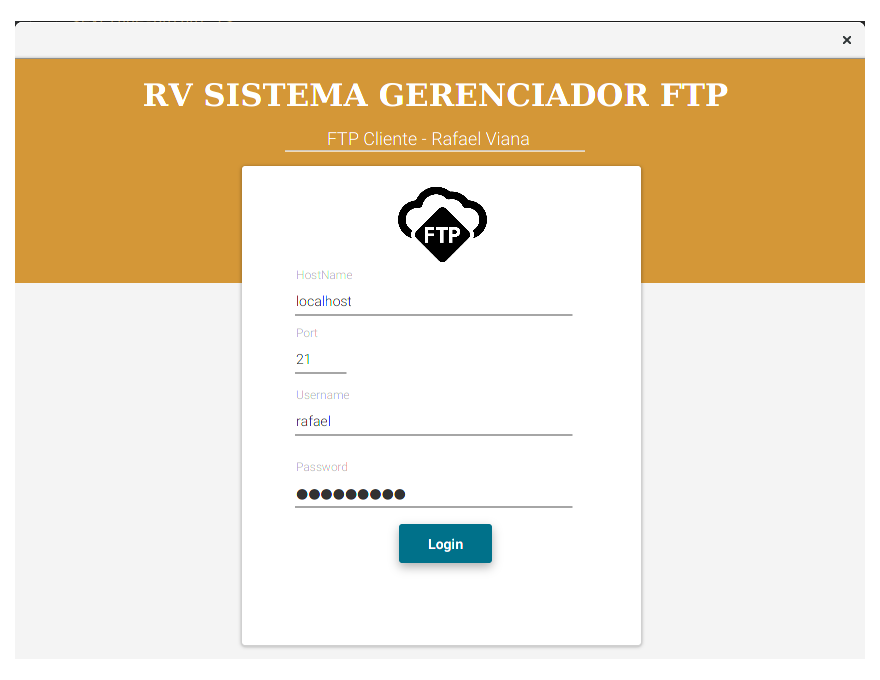
\includegraphics[width=1\textwidth]{Imagens/01.png}
	\caption{ Imagem da Tela de Login.}
	\label{fig:01}
\end{figure}

Com a tela de login aberta o usuário entra com as informações login , senha, endereço do host, port do host mostrado no código abaixo.

\begin{lstlisting}

private void login(ActionEvent event) {
	btnLogin.setVisible(false);
	imgProgress.setVisible(true);
	
	PauseTransition pauseTransition = new PauseTransition();
	pauseTransition.setDuration(Duration.seconds(3));
	pauseTransition.setOnFinished(ev -> {

try {
	
	int reply = FTPFactory.getInstance().FTPConecta(txtHostName.getText(),Integer.parseInt(txtHostPort.getText()),this.txtUsername.getText(),this.txtPassword.getText());
	System.out.println("Igual:" + reply);
	
	if (reply == 230) {
	
		btnLogin.getScene().getWindow().hide();
		completeLogin();
	
	} else {
	
		imgProgress.setVisible(false);
		btnLogin.setVisible(true);
		JOptionPane.showMessageDialog(null,"Erro Senha ou Usuário incorreto !!", "Erro ao Logar",JOptionPane.ERROR_MESSAGE);
	}

} catch (IOException ex) {
	Logger.getLogger(LoginController.class.getName()).log(Level.SEVERE, null, ex);
} catch (Exception ex) {
	Logger.getLogger(LoginController.class.getName()).log(Level.SEVERE, null, ex);
}

});
  pauseTransition.play();
}

private void completeLogin() throws IOException {
	
	imgProgress.setVisible(false);
	Stage dashboardStage = new Stage();
	dashboardStage.setTitle("");
	Parent root = FXMLLoader.load(getClass().getResource("Navegador.fxml"));
	Scene scene = new Scene(root);
	dashboardStage.setScene(scene);
	dashboardStage.show();
	
}
\end{lstlisting}
Após validar os dados de usuário a tela de navegação de documentos e aberta, essa tela nada mais é do que um conjunto de botões em uma Grid e um TreeView do JavaFX.


\begin{figure}[H]
	\centering
	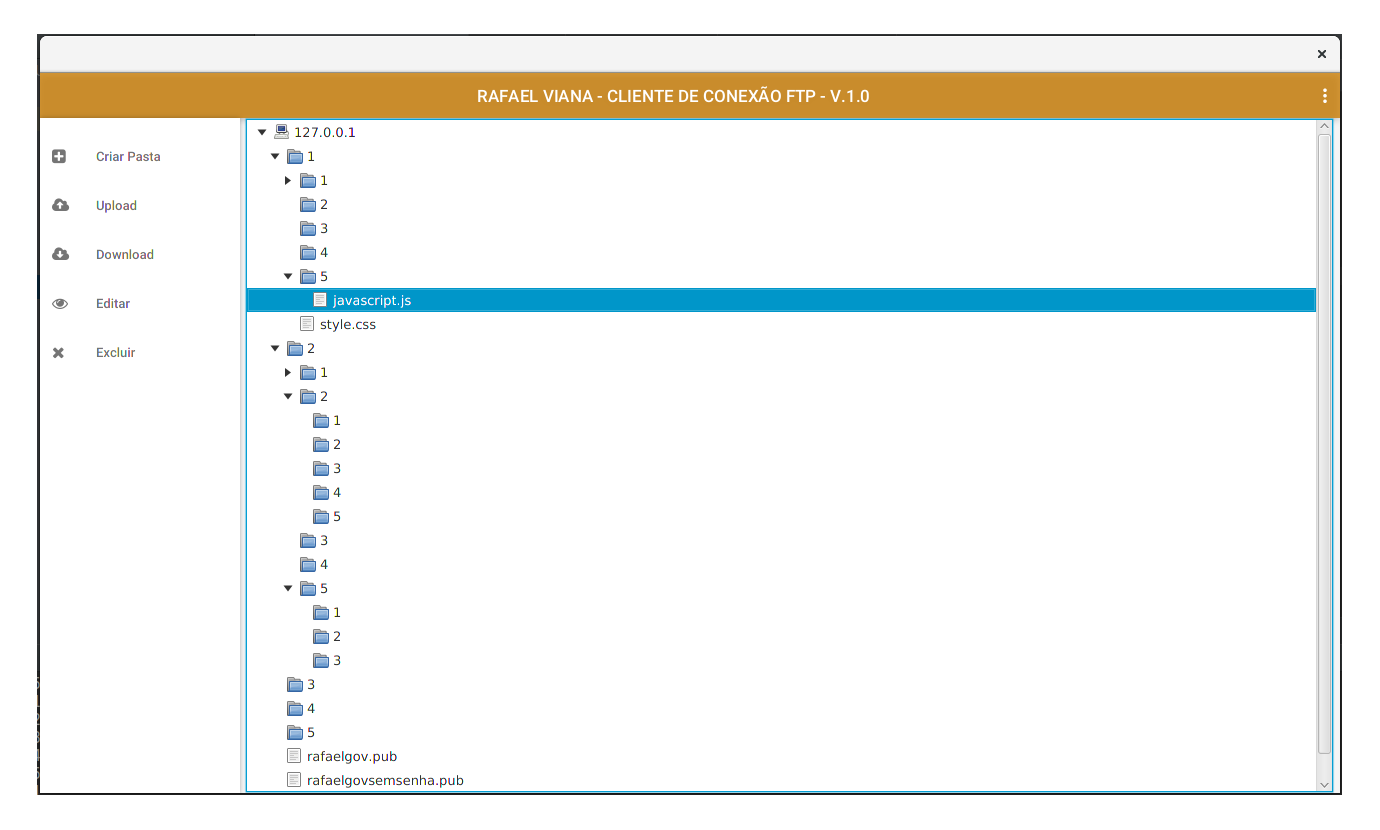
\includegraphics[width=1\textwidth]{Imagens/02.png}
	\caption{ Imagem da Tela de Navegação.}
	\label{fig:01}
\end{figure}

Para poder realizar a comunicação entre as classes e o FTPClient da apache, foi criado uma classe chamada de FTPFactory onde cria uma getInstance de FTPClient, podendo ser chamada de qualquer classe sem ter que que ser instanciada novamente, oque iria ocasionar a perda da conexão FTP.

\begin{lstlisting}
public class FTPFactory {
	
	private final FTPClient ftp;
	private TreeItem<FTPFile> file;
	private FTPFactory() {
		this.ftp = new FTPClient();
	}
	
	public static FTPFactory getInstance() {
		
		return FTPFactoryHolder.INSTANCE;
	}
	
	
	/**
	* Classe privada que armazena a única instância de FTPFactory.
	*/
	private static class FTPFactoryHolder {
		
		private static final FTPFactory INSTANCE = new FTPFactory();
	}
	
	
	
	public FTPClient getFTP(){
		return this.ftp;
	}
	
	
	public boolean Excluir(FTPFile file){
		try {
			if(file.isDirectory()){
				System.out.println(file.getLink());
				return    ftp.removeDirectory(file.getLink());
			}else{
				System.out.println(file.getLink());
				return   ftp.deleteFile(file.getLink());
			}
		} catch (IOException e) {
			e.printStackTrace();
			
		}
		return false;
	}
	
	
	public int FTPConecta(String host,int port, String user, String pwd) throws Exception {
		int reply;
		ftp.connect(host,port);
		reply = ftp.getReplyCode();
		if (!FTPReply.isPositiveCompletion(reply)) {
			ftp.disconnect();
			throw new Exception("Exception in connecting to FTP Server");
		}
		ftp.login(user, pwd);
		reply = ftp.getReplyCode();
		ftp.setFileType(FTPClient.BINARY_FILE_TYPE);
		ftp.enterLocalPassiveMode();
		ftp.setAutodetectUTF8(true);
		return reply;
	}
	
	
	
	
	public void disconnect() {
		if (this.ftp.isConnected()) {
			try {
				this.ftp.logout();
				this.ftp.disconnect();
			} catch (IOException f) {
				
			}
		}
	}
	
}
\end{lstlisting}




\end{document}


